\documentclass[a4paper,11pt]{article}
\usepackage[english]{babel}
\usepackage{amsmath}
\usepackage{amssymb}
\usepackage{amsthm}
\usepackage{array}
\usepackage{graphicx}
\usepackage{float}
\usepackage{placeins}
\usepackage{booktabs,caption,fixltx2e}
\usepackage[flushleft]{threeparttable}
\usepackage[margin=1in]{geometry}
\usepackage[utf8]{inputenc}

\title{\textbf{Managing Labs} \\ \large MSc Computing \& Information Technology}
\author{Jack McLean \bf190025023 \\ Supervisor: Ruth Letham}
\date{2020/2021}

\begin{document}
\maketitle
\begin{center}

\includegraphics[width = 2cm]{crest.png}
\end{center}

\newpage
\section*{Abstract}

\section*{Declaration}

\newpage
\tableofcontents

\newpage
\section{Introduction}

The following section outlines the background of this MSc dissertation. TODO ??? The existing methods and tools shall justify the motivation behind this project. 

\subsection{Background}

The School of Computer Science at the University of St. Andrews has historically run lab sessions for early years students, offering them support in developing their practical programming skills. The school traditionally operated these labs using a ‘hands-up’ system to organise in-class support, however the school's relatively rapid growth in class size means that this method is becoming less efficient. The global pandemic has further accelerated the need for an alternative support system, since the in-person labs replacement with online sessions meant that the traditional system was not possible. 


\subsection{Objectives}

The overall goal of this project is to create a custom system for the School that can be used to manage students' requests for practical programming assistance, both in virtual and physical lab sessions. 

TODO ??

\newpage
\section{Context Survey}

\subsection{Lab History ??}

30 people -> 200 people. 1 to 30 1 to 20 staff ratio, here are the needs identified, 


This chapter shall discuss and review the existing work around this project. The first section of this chapter investigates the current system used by school. The second section of this chapter contains an investigation into existing tools and systems that are available.

\subsection{Current System}

The current system for managing online lab sessions was developed and adapted at short notice due to the global pandemic. The initial solution was to create a `CS1000 Labs' team on Microsoft Teams \cite{teams}, the University's standard collaboration tool for online learning, and manage the lab sessions by posting announcements when labs opened. Students were then able to post new conversations under these announcements, which prompted them to tag the class demonstrators, and briefly summarising their issue and provide module code and practical number associated with their issue.

TODO: its not excel, microsoft lists?

TODO: power automate flows owned by system admin, in control of them/nobody else can access them,

TODO: maintenance locations, complicated sharepoint/automate

\FloatBarrier
\begin{figure}[H]
  \centering
  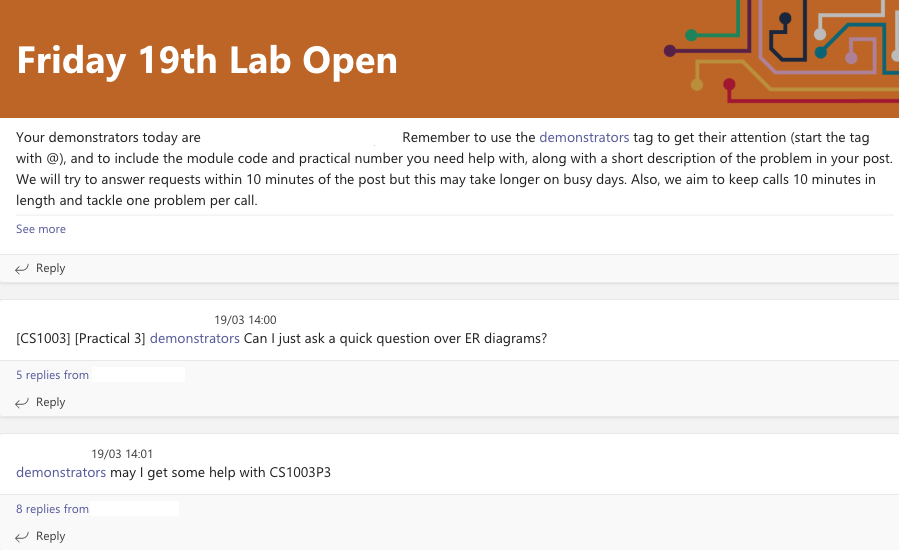
\includegraphics[width=\textwidth]{teams1.png}
  \caption{An example of the first iteration process of managing online labs.}
\end{figure}

The second, and current, iteration of the current system uses a form input. This is accessed using a `Request Form' tab in the Microsoft Teams \cite{teams} CS1000 Labs team. 

\FloatBarrier
\begin{figure}[H]
  \centering
  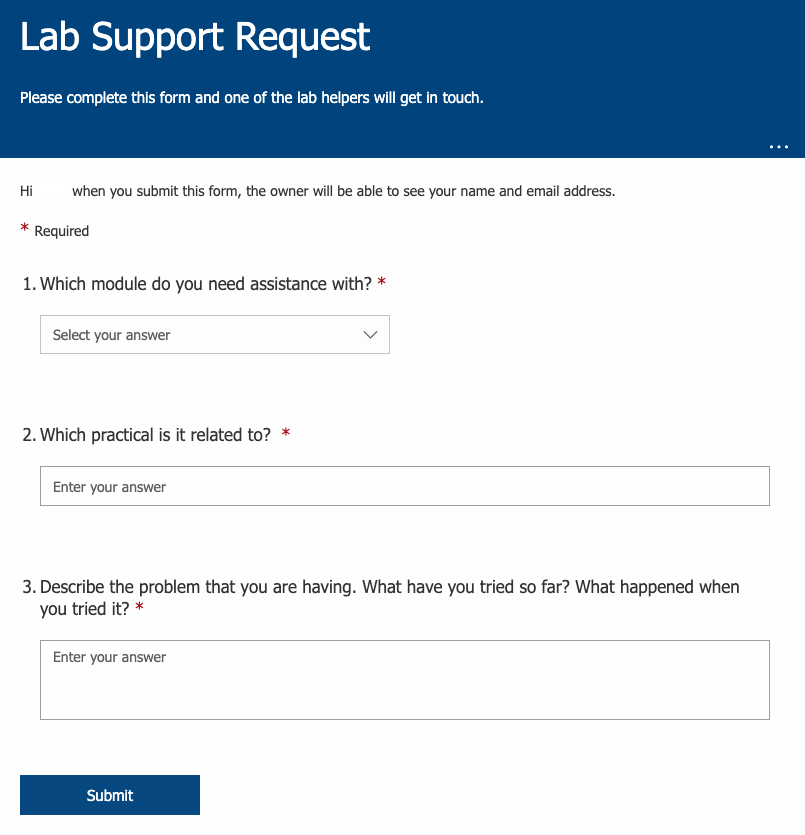
\includegraphics[width=0.85\textwidth]{teams2a.png}
  \caption{The request form from the second iteration process of managing online labs.}
\end{figure}

The form uses Power Automate \cite{pauto} to post on a private demonstrator team channel (used only to create a notification for class demonstrators) and add the form data to a Microsoft Excel spreadsheet. On this real-time collaborative spreadsheet, class demonstrators can assign themselves to students' requests before they make contact with the student through Microsoft Teams \cite{teams} or email. 

TODO notes:
\begin{itemize}
  \item email about closure collected from teams
  \item communication in video or text (depending on issue complexity) but both on teams
  \item is forms swimlane necessary? inbuilt on teams but also excel could be considered the same
\end{itemize}

\FloatBarrier
\begin{figure}[H]
  \centering
  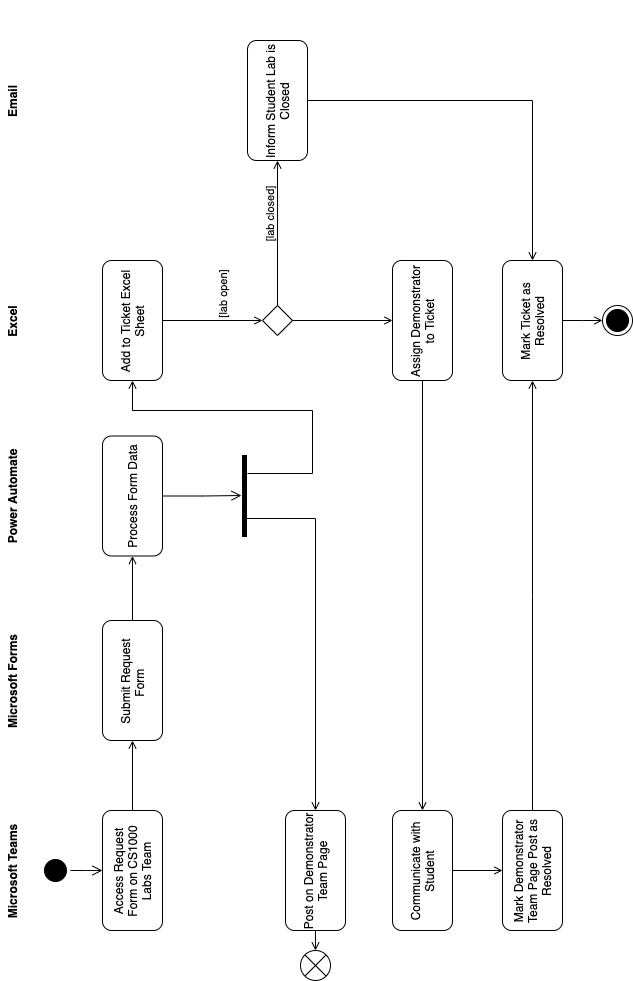
\includegraphics[width=0.95\textwidth]{activityPostExisting.png}
  \caption{Activity diagram for existing method of managing student online lab request.}
\end{figure}

\subsubsection{Software Evaluation}

- TODO algorithm not in order

\paragraph{Accessibility}
The current system meets the end user basic needs reasonably well. As a result of its integration with Microsoft Teams \cite{teams}, the form and navigation to it meet standard accessibility requirements \cite{formaccess} \cite{teamsaccess}. TODO worth mentioning this ? should this be a category?


\paragraph{Functionality}
For students, the functionality of the software is adequate. The form provides a method of posting issues to demonstrators. However, there are some further areas of functionality that the current system fails. The form does not given any indication of how busy the current lab is. Also, there are no means to withdraw a form from the demonstrators' excel sheet after posting. Further, the lab form allows students to post tickets outwith lab hours, meaning that they may wait some time (expecting a solution) before receiving a manual response about the lab being closed. Additionally, there is no simple way to access the help that other students received for similar issues - although an FAQ tab exists in Microsoft Teams \cite{teams}, it requires manual recognition of common problems and updating, meaning that the amount of solutions collected is significantly lower than with an automated system. 
        
For class demonstrators, the functionality is fairly adequate. The excel spreadsheet contains information on posted student issues, with the bonus of real-time updates from other demonstrators. There are functionality pitfalls for demonstrators too. One comes from the fact that the request form does not require much information about the problem, for example a minimum length of description or issue category, meaning that demonstrators do not have a lot of information before speaking to the student. Also, there is no functionality regarding lab opening hours - meaning that demonstrators must manually reply to all requests posted outwith lab hours.

For lab leads, there is no additional functionality. Lab leads must manually analyse the excel spreadsheet or Microsoft Teams \cite{teams} channel in order to gain further information. 

\paragraph{Performance}  
When used correctly by both class demonstrators and students, the system performs basic functionality well. The issue with the system is that it consists of multiple communicating platforms, however each platform is owned and maintained to a high standard by Microsoft. Performance issues could arise if applications were to be updated.

\paragraph{Ease of Use} 
For students, the system is fairly self explanatory and easy to use. Students simply access the form, provide information and then wait to be contacted by class demonstrators.

For class demonstrators, the system is more difficult to use. Since the system is comprised of multiple platforms, each must be considered when running a lab. For example, the demonstrators are notified of a new issue in Microsoft Teams \cite{teams}, the issue ticket is located in an excel spreadsheet and then communication with the student must be carried out in teams and/or email. It is worth nothing that the increased number of platforms increase the surface area for human error.


\paragraph{Customisation} 
Customisation in this system is reasonable. The form input fields and therefore the excel spreadsheet labels are customisable. The power automate \cite{pauto} flows (non-code scripts) are also customisable, however only within the limits of Microsoft's provided actions and applications.

\paragraph{Compatibility}  
The form is located in teams, along with the spreadsheet of issues for demonstrators. Communication is also carried out mostly using either the comment or video call features within Microsoft Teams. Since Microsoft Teams is the University wide standard collaboration tool for online learning, and is integrated with the University's Shibboleth \cite{shib} single sign-on platform, students should already have the technology installed and working on their machines. Additionally, the Microsoft Teams mobile application and form enable students to easily post tickets from their mobile devices.

TODO: cite teams every time ???

\paragraph{Robustness}
Robustness is where the current system fails. As discussed previously and conveyed in the activity diagram, the system is comprised of multiple, interlinked applications as well as manual input. If any of the applications are updated, down or behaving in an unexpected way then the system could fail to function - this could be difficult to detect in quieter labs and result in students waiting indefinitely on a response.


\paragraph{Cost}  
The current system is not free, however is covered by existing Microsoft Office licensing purchased by the university.  


\newpage
\subsection{Classroom Management Tools}

ClassroomQ is an existing classroom management tool. It offers a very simple system, where teachers can create a classroom which students can join, type a message and hit an `Assistance Needed' button to join the queue of students who need help. The basic process is shown below.

Firstly, the teachers start a classroom session.

\FloatBarrier
\begin{figure}[H]
  \centering
  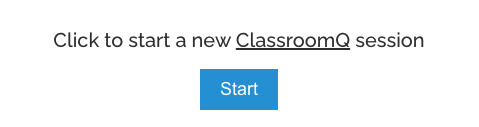
\includegraphics[width=0.5\textwidth]{cq1.png}
  \caption{Teacher's screen when a class has not been started.}
\end{figure}

The classroom is created, showing the class code which students can use to join.

\FloatBarrier
\begin{figure}[H]
  \centering
  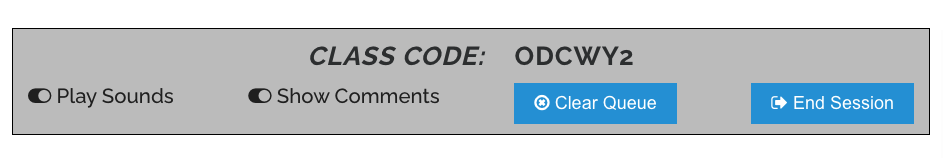
\includegraphics[width=0.75\textwidth]{cq2.png}
  \caption{Real time classroom queue, showing class join code and current requests.}
\end{figure}

Students join by entering their name and class code.

\FloatBarrier
\begin{figure}[H]
  \centering
  
\includegraphics[width=0.5\textwidth]{cq3.png}
  \caption{Student join page, showing sample class code and name.}
\end{figure}

Below is the image shown to students once they have joined the class. From this page they are able to type details of their problem in the comment section and then click the `Assistance Needed' button to join the queue.

\FloatBarrier
\begin{figure}[H]
  \centering
  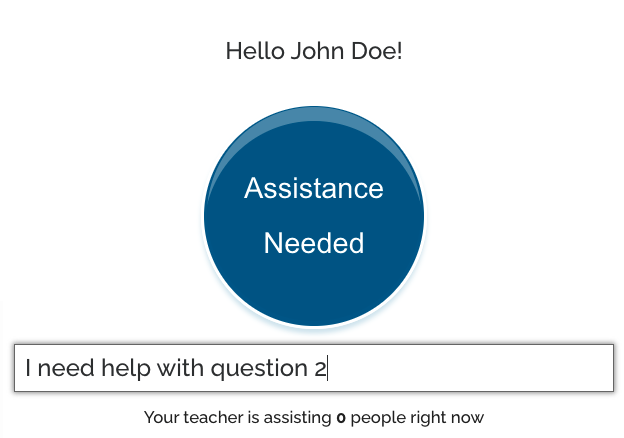
\includegraphics[width=0.5\textwidth]{cq4.png}
  \caption{Student help request page.}
\end{figure}

Once the student has joined the queue, they are taken to the page below. This allows them to cancel their request as well as providing real time information about their position in the queue.

\FloatBarrier
\begin{figure}[H]
  \centering
  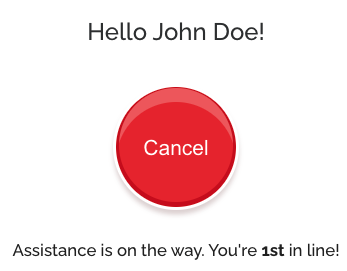
\includegraphics[width=0.5\textwidth]{cq5.png}
  \caption{Student page after posting help request.}
\end{figure}

The teacher is then able to see an ordered view of the student's requests in on the class page.

\FloatBarrier
\begin{figure}[H]
  \centering
  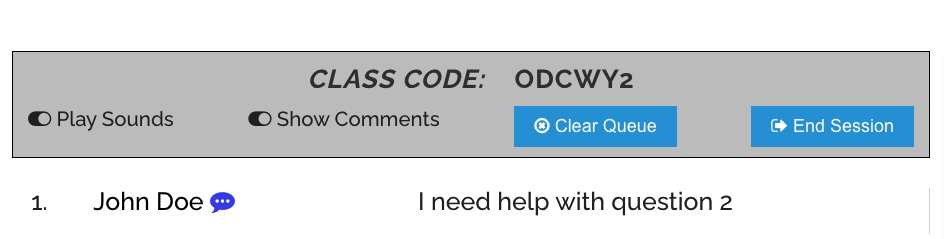
\includegraphics[width=0.75\textwidth]{cq6.png}
  \caption{Teacher's class page view after the request has been posted.}
\end{figure}


\subsubsection{Software Evaluation}

\paragraph{Functionality}
The website provides similar functionality to what we require in terms of being able to post issues, however is not suitable for a number of reasons.

For students, the amount of information they can provide is extremely limited. Only a single comment box, with a maximum of 190 characters, is available and therefore restricts students from providing a detailed description of their issue. There is also no prompt for any class or issue category information. Students are also unable to have more than one live request at a time. It is useful for all parties that the class sessions can be ended - stopping requests for help being posted outwith lab hours.

For class demonstrators, only a single account can be used - the system does not allow classes to have multiple teachers. This alone makes the application unsuitable, since there is no way to organise which demonstrator is assigned to which task. The system does not contain any integrated communication methods of any type. The system's method of obtaining student names is also unsuitable for managing school labs, since students could provide any form of name - something that would introduce issues when attempting to communicate with the student on a different system. Teacher accounts are also only able to, forever, open a single class with a persistent class code, meaning that running multiple labs or different labs is not possible.

For lab leads, no functionality exists that is separate from class demonstrators. However, it is possible to export logs of students who joined, as well as their help requests, which could be analysed in another platform.


\paragraph{Performance}  
It is hard to give an assessment of the system without it having been used in class. However, the application is fairly lightweight and has simple functionality so it is hard to foresee performance issues. TODO worth keeping this in?

\paragraph{Ease of Use}
The system's simplicity makes it extremely easy and intuitive to use. It is also possible to use the application on mobile. 

It is worth noting that for use in managing the University labs, this software would require communication on a different platform. Since the application does not enforce, or allow the enforcement of, validation of names, it would be difficult to find students on third party applications.


\paragraph{Customisation} 
The application provides no options for customisation of any kind.


\paragraph{Compatibility}  
Being web based means that students are not required to download and install any third-party software. 


\paragraph{Robustness}
As with performance, it is hard to give an assessment of the system without it having been used in class. It is, again, reasonable to expect that the application is fairly robust given its simplicity.


\paragraph{Cost}  
The system offers multiple membership levels which cost varying amounts. The level that would be required for the University of St.\ Andrews would be \$12.99 per year per teacher, for a minimum of 5 teacher accounts.


\newpage
\subsection{Incident Management Tools}

Spiceworks Cloud Help Desk is a free to use, cloud-based help desk that is used by IT professionals. Traditionally, the system is used to track and manage IT issues in order to provide IT support, however the system could also be used to track and manage requests for help in our lab management domain. The basic process is shown below.

Firstly, students would access a link to the help portal and enter their email address.

\FloatBarrier
\begin{figure}[H]
  \centering
  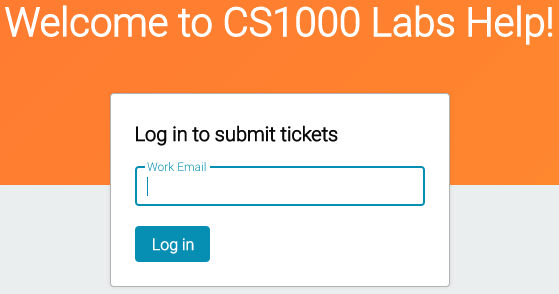
\includegraphics[width=0.5\textwidth]{SWportalLogin.png}
  \caption{Login screen from portal link.}
\end{figure}

The student would then, if authorised, receive an email link to login to the portal. This would take them to the following form.

\FloatBarrier
\begin{figure}[H]
  \centering
  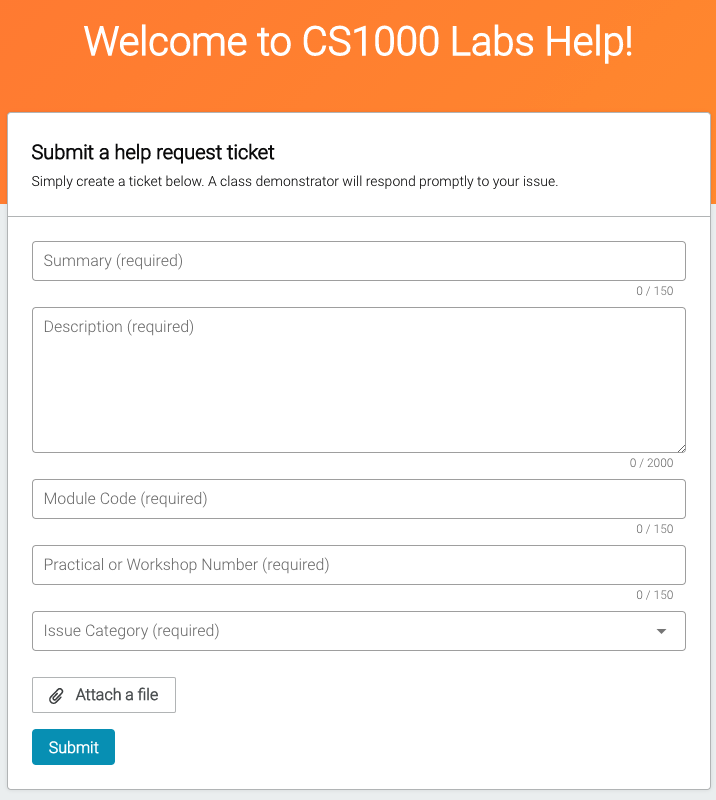
\includegraphics[width=0.65\textwidth]{SWpostTicket.png}
  \caption{Ticket posting form, reached after login.}
\end{figure}

The ticket would then appear on the class demonstrator help desk.

\FloatBarrier
\begin{figure}[H]
  \centering
  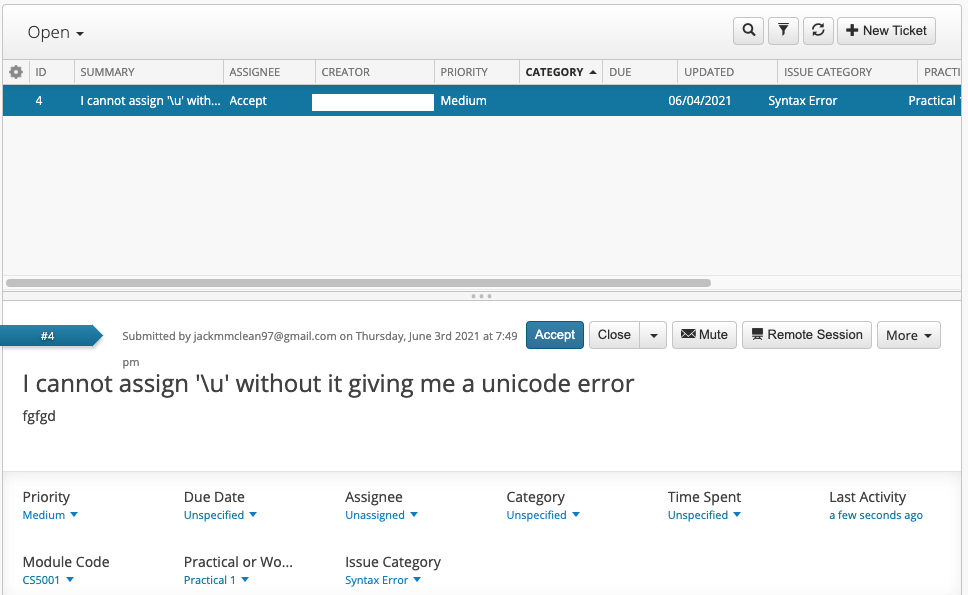
\includegraphics[width=0.85\textwidth]{SWticketPage.png}
  \caption{The help desk ticket page, accessible to class demonstrators.}
\end{figure}

Class demonstrators are then able to respond to the ticket on Spiceworks, notifying the user by email, and initiate a video call on a different service if necessary. The demonstrator can then close the ticket when complete.

\subsubsection{Software Evaluation}

\paragraph{Functionality}
For students, spiceworks is functional to the point that we require for our system. The system allows tickets to be created via a customisable user portal, which can be modified to include module code, practical number and issue category in text field, text area and select inputs. The system also allows tickets to be posted by email. One issue with functionality is that some attributes are `baked-in' to the system, for example it is not possible to remove the `summary' or `description' input fields from the ticket posting form. Additionally, the system has a due date attribute for tickets that cannot be removed.

For class demonstrators, the ticket management UI functions well. It allows tickets to be assigned, edited, closed, merged with other tickets. The system also has a useful `last activity' attribute on each ticket. The privacy controls on the user portal also allow an `active directory' to be created, something that would be useful in authenticating to ensure users are students. A timeline feature on the system also shows demonstrators a time sorted list of all activities. There is no way to distinguish between tickets that have been resolved or closed unsuccessfully. 

For lab demonstrators, a useful summary dashboard is provided. This provides useful infographs and key statistics such as average first response time, average ticket close time, ticket category breakdown and top ticket creators. It does not provide any information on specific class demonstrators, however Spiceworks allows the generation of summary reports which can be produced for each individual demonstrator. The system also does not have any option to prevent tickets being posted outwith lab hours, although this information could be added to an autmatic email response. It is also important to note that there are no different admin roles on Spiceworks - functionality does not differ between class demonstrators and lab leads.


\paragraph{Performance}
As with ClassroomQ, it is hard to comment on the domain specific performance. However, Spiceworks is an established, popular ticketing system and therefore a reasonable level of performance would be expected. 


\paragraph{Ease of Use} 

The system is fairly simple and intuitive to use for students. The administrative aspect is slightly more complex, however would be quick and easy to learn after the initial setup. One issue is that the system is designed for tech issue ticketing, therefore some of the application and documentation language refers specifically to that domain.

\paragraph{Customisation} 

The system is fairly customisable. It also different form attributes to be added to the user portal, therefore also to the tickets. There is no option to customise other aspects of the system, such as the summary dashboard


\paragraph{Compatibility}  

This system has the advantage of being web based, meaning that users do not need to download and install third party content. It is also possible to import and export tickets in JSON form, meaning that tickets could be easily migrated to or from the system.

\paragraph{Robustness}
As with performance, it is hard to give an assessment of the system without it having been used in class. It is, again, reasonable to expect that the application is fairly robust given its popularity.


\paragraph{Cost}  
All Spiceworks products are entirely free. They are, however, funded by advertising revenue which is generated by selling data stored on Spiceworks. This could be a serious issue for the lab management domain, as students would be well within their right to refuse the service. Another problem is that Spiceworks terms of use specifies that organisations must obtain permission to use the service.

\newpage
\section{Design}

\newpage
\subsection{User Stories}

\newpage
\subsection{System Requirements}

TODO stakeholders ?

TODO MOSCOW PRIORIT - must, should, ought, would, wont, could

\subsubsection{Functional Requirements}

\begin{table}[H]
\small
\begin{tabular}{|p{0.05\linewidth} | p{0.78\linewidth} |p{0.09\linewidth}|}
 \hline
 \textbf{ID} & \textbf{Details} & \textbf{Priority} \\
 \hline
 
 \multicolumn{3}{c}{\textit{\textbf{Account Requirements}}}\\
 
 \hline
 F-01 & \textit{Description:} The system shall allow students to register on the system by providing a verified student email address and a password. & High\\
  \cline{2-2}
  & \textit{Rationale:} Students must be able to sign up using only a school email address, which they can verify access to, to register on the system. & \\

  
   \hline\hline
 F-02 & \textit{Description:} The system should allow students to sign in using the Shibboleth SSO system used by the school. & Low\\
  \cline{2-2}
  & \textit{Rationale:} Students can only log in if Shibboleth authenticates them, making the system more secure, reliable and meaning authentication is centralised to align with other school systems. & \\

  
     \hline\hline
 F-03 & \textit{Description:} Lab leads shall be able to assign class demonstrator role to users. & High\\
  \cline{2-2}
  & \textit{Rationale:} This allows class demonstrator accounts to be created without allowing regular students to attempt to class create demonstrator accounts. & \\

  
       \hline\hline
 F-04 & \textit{Description:} System administrators shall be able to assign lab lead role to users. & High\\
  \cline{2-2}
  & \textit{Rationale:} This allows lab lead accounts to be created. & \\
  \hline
  
   \multicolumn{3}{c}{\textit{\textbf{Ticket Requirements}}}\\
  
 \hline
 F-05 & \textit{Description:} Whilst the lab is open, students shall be able to create `tickets' by providing information on the module code, practical or workshop number, issue category and issue description. & High\\
  \cline{2-2}
  & \textit{Rationale:} This creates a record of the issue that the student is having for the class demonstrators to interact with. & \\

  
 \hline\hline
 F-06 & \textit{Description:} Students should be able to add tags to their own tickets which associate them with related tickets. & Medium\\
  \cline{2-2}
  & \textit{Rationale:} This allows students to give more clarification about the nature of the problem, create links with similar tickets (which they can view) and also help the system recommendation algorithm recommend similar past tickets. & \\

  
    \hline\hline
 F-07 & \textit{Description:} The system should recommend similar archived tickets before students post their tickets. & Low\\
  \cline{2-2}
  & \textit{Rationale:} This allows students to scan archived tickets, checking if any will help resolve their issue, before they post a live ticket that demonstrators need to deal with. & \\
  
      \hline\hline
 F-08 & \textit{Description:} The system should keep a record of which archived tickets students have selected (`this solved my problem') before deleting the original ticket draft. & Low\\
  \cline{2-2}
  & \textit{Rationale:} This allows lad leads and demonstrators to get information on issues which multiple students have had. & \\
  
   \hline\hline
 F-09 & \textit{Description:} Class demonstrators shall be able to assign themselves to tickets. & High\\
  \cline{2-2}
  & \textit{Rationale:} This allows demonstrators to keep track of, and indicate to other demonstrators, which issues they are working on or have completed. & \\

  
  \hline\hline
 F-10 & \textit{Description:} Class demonstrators shall be able to comment on tickets. & High\\
  \cline{2-2}
  & \textit{Rationale:} This allows demonstrators to make notes on the issues and initiate contact with the students, although actual communication would primarily be done outside the system. & \\

    \hline\hline
 F-11 & \textit{Description:} Class demonstrators shall be able to close tickets. & High\\
  \cline{2-2}
  & \textit{Rationale:} This allows demonstrators to mark tickets as no longer being `live' - either marking them as resolved or closed. & \\

  
      \hline\hline
 F-12 & \textit{Description:} Students should be able to close tickets. & High\\
  \cline{2-2}
  & \textit{Rationale:} This allows students to remove their issues from the queue if they have solved the problem themselves. & \\
\hline



  \end{tabular}
\end{table}

\begin{table}[H]
\small
\begin{tabular}{|p{0.05\linewidth} | p{0.78\linewidth} |p{0.09\linewidth}|}
  
          \hline
 F-13 & \textit{Description:} Class demonstrators should be able to `open' the lab, allowing tickets to be created by students. & Medium\\
  \cline{2-2}
  & \textit{Rationale:} This allows demonstrators to prevent help requests outwith lab hours. & \\

  
\hline\hline
 F-14 & \textit{Description:} Lab leads should be able to ban or suspend users from the system. & Medium\\
  \cline{2-2}
  & \textit{Rationale:} This allows lab leads to remove users for inappropriate behaviour or posting excessively. & \\
 
 \hline\hline
 F-15 & \textit{Description:} The system should not allow offensive or abusive content to be posted. & Medium\\
  \cline{2-2}
  & \textit{Rationale:} Prevents offensive behaviour. & \\
 
 \hline\hline
 F-16 & \textit{Description:} The system should not allow students to post more than one ticket every 3 minutes. & Low\\
  \cline{2-2}
  & \textit{Rationale:} This prevents individual students from posting an excessive number of tickets on the system. TODO: should this be 3 minutes? limit to number of req per lab instead??? & \\
 
  \hline\hline
 F-17 & \textit{Description:} The system should allow students to edit and update their live tickets. & Medium\\
  \cline{2-2}
  & \textit{Rationale:}  This allows users to provide more information on a ticket to improve demonstrators ability to help them. & \\
 
   \hline\hline
 F-18 & \textit{Description:} The system shall have an integrated live chat feature on each ticket that has a demonstrator assigned. & Medium\\
  \cline{2-2}
  & \textit{Rationale:} This allows students and demonstrators to briefly discuss minor issues or to arrange communication outside the system. & \\

   \hline\hline
 F-19 & \textit{Description:} The system should have some form of video chat option on each ticket that has a demonstrator assigned. & Low\\
  \cline{2-2}
  & \textit{Rationale:} This allows students and demonstrators to resolve the problem raised by the ticket, removing any human error associated with looking the student up on another system - as well as reducing time spent doing so. & \\

   \hline\hline
 F-20 & \textit{Description:} The system should allow class demonstrators to post a `solution' for ticket. & Medium\\
  \cline{2-2}
  & \textit{Rationale:} This allows demonstrators to store solutions with archived tickets, useful for future reference when archived tickets are recommended as similar to future students' tickets. & \\

   \hline\hline
 F-21 & \textit{Description:} The system should prompt class demonstrators to provide solutions for archived tickets which have repeatedly been marked by students as similar to their own tickets. & Low\\
  \cline{2-2}
  & \textit{Rationale:} This encourages demonstrators to provide solutions for more common problems, ensuring the recommendation system will be useful and therefore reduce the number of new tickets being created. It is also useful for reference by other class demonstrators. & \\

  
     \hline\hline
 F-22 & \textit{Description:} The system should give some indication to students of how busy the current lab session is or how many tickets are ahead of them in the queue. & Medium\\
  \cline{2-2}
  & \textit{Rationale:} This allows students to appreciate the amount of wait time that a response may require. & \\

     \hline\hline
 F-23 & \textit{Description:} The system shall allow students to specify their location for in-person labs. & High\\
  \cline{2-2}
  & \textit{Rationale:} This allows the tool to be used for management of in-person labs, as well as labs which are both in-person and have virtual participants. & \\
 
      \hline\hline
 F-24 & \textit{Description:} The system should allow students to attach files to their tickets. & Medium\\
  \cline{2-2}
  & \textit{Rationale:} This allows demonstrators to study, understand and potentially solve issues quickly before they need to contact the student. & \\
  
        \hline\hline
 F-25 & \textit{Description:} The system should show class demonstrators and lab leads a `timeline' of all actions on the system - such as lab opening, ticket posting, ticket commenting, ticket resolution and lab closing. & Low\\
  \cline{2-2}
  & \textit{Rationale:} This allows demonstrators and lab leads to quickly scan recent activity, as well as helping demonstrators to quickly find recent tickets or comments. & \\
  \hline
 
 \end{tabular}
\end{table}
 
 \begin{table}[H]
\small
\begin{tabular}{|p{0.05\linewidth} | p{0.78\linewidth} |p{0.09\linewidth}|}
 
  \multicolumn{3}{c}{\textit{\textbf{Summary Requirements}}}\\
 
 \hline
 F-26 & \textit{Description:} Lab leads shall be able to view lab summaries which provide statistics about the amount of tickets resolved, who resolved tickets and how long tickets remained unresolved in each individual lab. & High\\
  \cline{2-2}
  & \textit{Rationale:} This allows lab leads to review the efficiency of the ticketing system in the lab. & \\

 \hline\hline
 F-27 & \textit{Description:} Lab leads shall be able to view class summaries which provide statistics about the amount of tickets resolved, who resolved tickets and how long tickets remained unresolved for all labs in a given class. & High\\
  \cline{2-2}
  & \textit{Rationale:} This allows lab leads to review the efficiency of the ticketing system in the class. & \\
  \hline
  
\end{tabular}
\end{table}

\subsubsection{Non-Functional Requirements}

\begin{table}[H]
\small
\begin{tabular}{|p{0.07\linewidth} | p{0.78\linewidth} |p{0.09\linewidth}|}
 \hline
 \textbf{ID} & \textbf{Details} & \textbf{Priority} \\
 
 \hline
   \multicolumn{3}{c}{\textit{\textbf{Usability Requirements}}}\\
 \hline
 
   NF-01 & \textit{Description:} 95\% of students should be able to create a ticket in less than 5 minutes on the first attempt. & Medium \\
  \cline{2-2}
  & \textit{Rationale:} The system should be intuitive, quick and easy to use. & \\

   \hline\hline
      NF-02 & \textit{Description:} 95\% of class demonstrators should be able to resolve a ticket, in the correct way (for example, marking the problem as resolved), in less than 1 minute on the first attempt. & Medium \\
  \cline{2-2}
  & \textit{Rationale:} The system should be intuitive, quick and easy to use. & \\
   \hline
     
     \multicolumn{3}{c}{\textit{\textbf{Security Requirements}}}\\
     
     \hline
 NF-03 & \textit{Description:} Data shall be encrypted. & High\\
  \cline{2-2}
  & \textit{Rationale:} Data needs to be protected from hostile users. & \\
  
    \hline\hline
 NF-04 & \textit{Description:} Data shall be stored securely. & High\\
  \cline{2-2}
  & \textit{Rationale:} Data needs to be protected from hostile users. & \\
  
      \hline\hline
 NF-05 & \textit{Description:} The system shall anonymise (and archive for future reference) all resolved tickets. & High\\
  \cline{2-2}
  & \textit{Rationale:} This allows the system to show users the archived tickets without processing or storing any personal data. & \\
  
      \hline\hline
 NF-06 & \textit{Description:} The system shall allow only class demonstrators (and lab leads) to view live tickets and names of students. & High\\
  \cline{2-2}
  & \textit{Rationale:} This addresses privacy concerns arising from students being able to view other students' names and tickets. & \\
\hline
  
    \multicolumn{3}{c}{\textit{\textbf{Performance Requirements}}}\\
    
  \hline
   NF-07 & \textit{Description:} Class demonstrator ticket assignment shall be processed and updated for other users within 0.1s. & High \\
  \cline{2-2}
  & \textit{Rationale:} Slow assignment processing and updating could result in issues with conflicting assignment and demonstrators working on the same ticket. & \\
 
   \hline\hline
   NF-08 & \textit{Description:} Resolution of tickets shall be processed and updated for other users within 1s. & Medium \\
  \cline{2-2}
  & \textit{Rationale:} Ticket resolution should be processed reasonably quickly to prevent lab leads following up tickets resolved by demonstrators or demonstrators following up tickets resolved by students. & \\
  \hline
  
      \multicolumn{3}{c}{\textit{\textbf{Dependability Requirements}}}\\
  
   \hline
   NF-09 & \textit{Description:} The System shall achieve 99\% up time. & High \\
  \cline{2-2}
  & \textit{Rationale:} Since students rely on the labs for help and they are only open for a small amount of time, it is critical that down time during the lab window is reduced. & \\
\hline
   
\multicolumn{3}{c}{\textit{\textbf{Space Requirements}}}\\
   
   \hline
   NF-10 & \textit{Description:} The system should be able to store at least 100,000 tickets. & Medium \\
    \cline{2-2}
  & \textit{Rationale:} Since there are many labs for each module, which involves multiple practicals, it is important that the archive is capable of storing tickets for future reference. & \\
 \hline

\end{tabular}
\end{table}

\newpage
\subsection{Use Case}

\subsubsection{Use Case Diagram}

\begin{figure}[H]
    \centering
    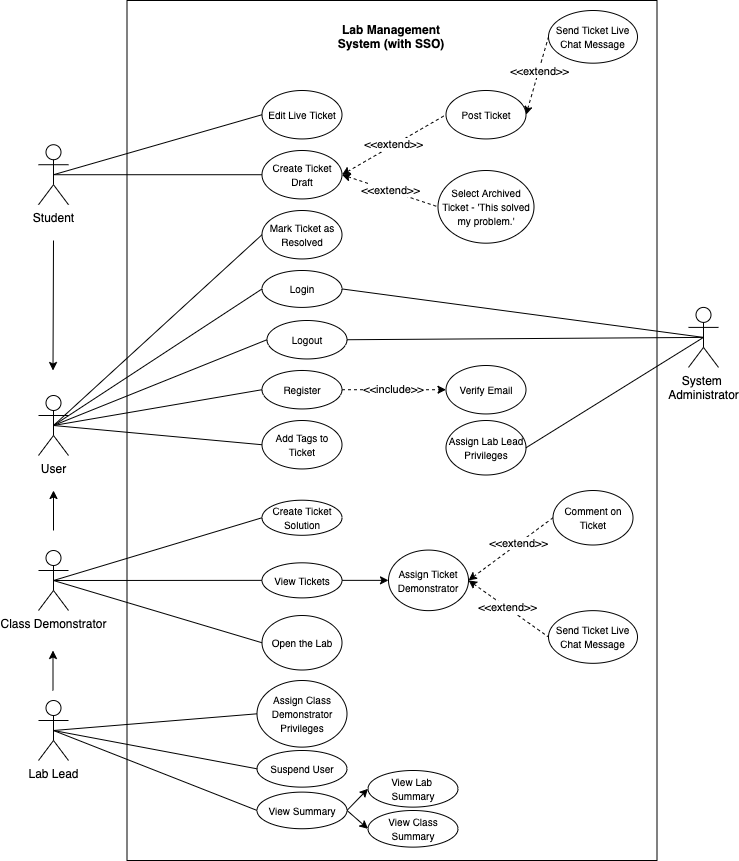
\includegraphics[width=\textwidth]{useCase.png}
    \caption{Use case diagram for lab management system.}
    \label{fig:useCase}
\end{figure}

\subsubsection{Use Case Specifications}

\subsubsection*{`Create Ticket Draft' Use Case Specification}
\begin{table}[H]
\centering
 \begin{tabular}{p{0.27\linewidth}  p{0.67\linewidth}}
 \textbf{Use case name} & \textbf{Post Ticket}  \\
 Use case ID & 1\\
 Brief Description & A student creates a ticket draft on the system.\\
 Preconditions & The student is a registered and verified, the lab is open.\\
 Primary actors & Student. \\
 Secondary actors & \textbf{None.} \\
 Successful end condition & A new live ticket is posted onto the system for class demonstrators to view. \\
 Failed end condition & The ticket listing is rejected. \\
 Main flow & Steps:\\
 & 1. The use case starts when a student tries to visit the `post a ticket' page.\\
 & 2. The system checks that the user is logged in as a registered, verified account with student role privileges. \\
 & 3. The `post a ticket' page is opened. \\
 & 4. The student inputs the details of the issue - associated module, relevant practical or worksheet, the issue category and a description issue.\\
 & 5. The student submits the information. \\
 & 6. The system checks that the student has not posted a ticket in the last 3 minutes. \\
 & 7. The system checks that the ticket does not contain offensive or abusive language. \\
 & 8. The system checks that no archived, resolved tickets are highly similar to the draft ticket.\\
 & 9. The new ticket is posted on the application.\\

 Extension & Step\hspace{0.3cm} Branching Action \\
 & 2.1 \hspace{0.5cm}The user is not logged in as a registered, verified student. \\
 & 2.2 \hspace{0.5cm}Access to the `post a ticket' page is denied. \\
 & 6.1 \hspace{0.5cm}The student has posted a ticket in the last 3 minutes. \\
 & 6.2 \hspace{0.5cm}The system does not post the ticket, shows an error message modal. \\
 & 7.1 \hspace{0.5cm} The ticket contains offensive or abusive language.\\
 & 7.2 \hspace{0.5cm} The system does not post the ticket, shows an error message modal and logs the ticket for review by a lab lead.\\
 & 8.1 \hspace{0.5cm} The draft ticket is highly similar to one or more archived, resolved tickets.\\
 & 8.2 \hspace{0.5cm} The system allows the student to view the similar ticket(s).\\
 & 8.3 \hspace{0.5cm} The student selects `this solved my problem' on a ticket.\\
 & 8.4 \hspace{0.5cm} The system records the selection of the archived ticket and discards the student's draft ticket.\\
 & 8.3.1 \hspace{0.5cm} The student selects `this does not help'.\\
 & 8.3.2 \hspace{0.5cm} The new ticket is posted on the application.\\
 
\end{tabular}
\end{table}

\newpage
\subsubsection*{`Resolve Ticket' Use Case Specification}
\begin{table}[H]
\centering
 \begin{tabular}{p{0.27\linewidth}  p{0.67\linewidth}}
 \textbf{Use case name} & \textbf{Resolve Ticket}  \\
 Use case ID & 2\\
 Brief Description & A class demonstrator resolves a student's issue ticket.\\
 Preconditions & The ticket is live and not assigned to any class demonstrators.\\
 Primary actors & Class Demonstrator. \\
 Secondary actors & Student. \\
 Successful end condition & The ticket is marked as resolved. \\
 Failed end condition & The ticket is mark as closed but unresolved. \\
 Main flow & Steps:\\
 & 1. The use case starts when a class demonstrator attempts to visit the live tickets page.\\
 & 2. The system checks that the user is logged in as a registered, verified account with class demonstrator role privileges. \\
 & 3. The live ticket page is opened and shows a queue of all unresolved, not closed tickets that were posted in the current lab. \\
 & 4. The class demonstrator selects a ticket in the queue.\\
 & 5. The class demonstrator assigns themselves to the ticket. \\
 & 6. The class demonstrator sends the student a live chat, either explaining the solution, asking for more information or requesting a video chat. \\
 & 7. The class demonstrator solves the student's problem and marks the issue ticket as resolved. \\
 & 8. The class demonstrator is given the option to store a solution to the problem on the system.\\
 & 9. The ticket is archived on the system.\\

 Extension & Step\hspace{0.3cm} Branching Action \\
 & 2.1 \hspace{0.5cm}The user is not logged in as a registered, verified class demonstrator. \\
 & 2.2 \hspace{0.5cm}Access to the live ticket page is denied. \\
 & 7.1 \hspace{0.5cm} The class demonstrator cannot solve the problem.\\
 & 7.2 \hspace{0.5cm} The ticket is closed, marked unresolved, and the system logs the ticket for review by a lab lead.\\
  
\end{tabular}
\end{table}


\newpage
\subsection{Sequence Diagram}

\newpage
\addcontentsline{toc}{section}{References}
\begin{thebibliography}{9}

\bibitem{teams}
Microsoft Teams.
{\textit{Microsoft}}. [ONLINE] Available at: https://www.microsoft.com/en-gb/microsoft-teams/group-chat-software

\bibitem{pauto}
Power Automate.
{\textit{Microsoft}}. [ONLINE] Available at:
https://flow.microsoft.com/en-us/connectors/shared\_teams/microsoft-teams/

\bibitem{formaccess}
Accessibility support for Microsoft Forms.
{\textit{Microsoft}}. [ONLINE] Available at:
https://support.microsoft.com/en-us/office/accessibility-support-for-microsoft-forms-a77e8a20-ce55-4f93-99a2-96bd688b86f3

\bibitem{teamsaccess}
Accessibility support for Microsoft Teams.
{\textit{Microsoft}}. [ONLINE] Available at:
https://support.microsoft.com/en-us/office/accessibility-support-for-microsoft-teams-d12ee53f-d15f-445e-be8d-f0ba2c5ee68f

\bibitem{shib}
Single sign-on (SSO).
{\textit{University of St. Andrews}}. [ONLINE] Available at: https://www.st-andrews.ac.uk/itsnew/newsletter/2009/09/sso.html

\end{thebibliography}
\end{document}

